\documentclass[aspectratio=1610,xcolor=dvipsnames,t]{beamer} 

\usepackage{listings} 
\usepackage{color} 
\usepackage{xcolor}  
\usepackage{microtype} 
\usepackage{helvet} 
\usepackage{inconsolata} 
\usepackage[framemethod=TikZ]{mdframed} 
\usepackage{graphicx} 
\usepackage{alltt}
\usepackage{sverb} 
\usepackage{verbatim} 
\usepackage{pifont} 
\usepackage{alltt} 
\usepackage{helvet} 

\usetheme{Madrid} 
\useinnertheme{rectangles} 

\setbeamertemplate{navigation symbols}{}
\setbeamertemplate{blocks}[default] 

%\definecolor{mypurple}{rgb}{.49,0,98}
%\setbeamercolor*{palette primary}{use=structure,fg=white,bg=green}
%\usecolortheme[rgb={0.9,0.2,0.2}]{structure}
%\usecolortheme[rgb={0.6,0.1,0.1}]{structure}
%\usecolortheme[rgb={0.4, 0.0, 0.4}]{structure} 
\usecolortheme[rgb={0.0, 0.5, 0.9}]{structure} 

\usepackage{color}
\definecolor{orange}{cmyk}{0,0.4,0.8,0.2}
\definecolor{darkorange}{rgb}{.71,0.21,0.01}
\definecolor{darkgreen}{rgb}{.12,.54,.11}
\definecolor{myteal}{rgb}{.26, .44, .56}
\definecolor{gray}{gray}{0.45}
\definecolor{lightgray}{gray}{.95}
\definecolor{mediumgray}{gray}{.8}
\definecolor{inputbackground}{rgb}{.95, .95, .85}
\definecolor{outputbackground}{rgb}{.95, .95, .95}
\definecolor{traceback}{rgb}{1, .95, .95}
\definecolor{inputbg}{rgb}{0.98, 0.98, 0.98}

\usepackage{listings} 
\lstset{language=c,
        %basicstyle=\footnotesize\ttfamily, 
        basicstyle=\small\ttfamily,
        columns=fullflexible, 
        %title=\lstname, 
        %numbers=left, stringstyle=\texttt, 
        %numberstyle={\tiny\texttt}, 
        keywordstyle=\color{blue}, 
        commentstyle=\color{darkgreen}, 
        stringstyle=\color{purple} } 


\mdfsetup{skipabove=\topskip, skipbelow=\topskip} 

\definecolor{codebg}{rgb}{0.99,0.99,0.99}

\global\mdfdefinestyle{code}{%
    frametitlerule=true,%
    frametitlefont=\small\bfseries\ttfamily,%
    frametitlebackgroundcolor=lightgray,%
    backgroundcolor=codebg,%
    linecolor=gray, linewidth=0.5pt,%
    leftmargin=0.5cm, rightmargin=0.5cm,%
    roundcorner=2pt,%
    innerleftmargin=5pt
}

\global\mdfdefinestyle{code2}{%
    topline=false,%
    bottomline=false,%
    leftline=true,%
    rightline=false,%
    backgroundcolor=codebg,%
    linecolor=gray, linewidth=0.5pt,%
    leftmargin=0.0cm, rightmargin=0.0cm,%
    innerleftmargin=1pt
}

\newcommand{\showcode}[1]{\begin{mdframed}[style=code] %
                            \lstinputlisting{#1}% 
                          \end{mdframed}% 
}

\newcommand{\showsmallcode}[1]{\begin{mdframed}[style=code] %
        \lstinputlisting[basicstyle=\ttfamily\tiny]{#1}% 
                          \end{mdframed}% 
}




\title[Introduction to OpenGL]{Introduction to OpenGL \textregistered}
\titlegraphic{\centering
\includegraphics[width=0.3\textwidth]{opengl-logo}}
\subtitle{Graphics and Computation} 
\author{Michael Papasimeon} % \\
\date[2006,2007,2008]{12 March 2006\\
      11 March 2007\\
      11 March 2008} 

\begin{document}

\begin{frame}
    \titlepage
    \footnote{\tiny OpenGL® and the oval logo are trademarks or registered trademarks of Silicon Graphics, Inc. in the United States and/or other countries worldwide.} 
\end{frame} 

\begin{frame}{Notes}  
    \begin{itemize} 
    \item These slides were presented to a third year computer science class in
        graphics and computation over a three year period (2006, 2007, 2008). 
        The slides were the practical component introducing the students to
        OpenGL as part of a longer course in computer graphics. 
        The introductory OpenGL component was taught over two lectures, but
        the students used OpenGL for the major project. 
    \item There was some variation over the three years in which the material
        was presented, including one year (2007) where Java was used with JOGL.
        In 2006 and 2008 the course was taught in C using GLUT. 
    \item The slides were originally done in PowerPoint and they have been
        convertex to \LaTeX and Beamer. 
    \end{itemize} 
    \begin{alertblock}{OpenGL Version} 
        Note that the OpenGL presented in these slides is pretty out of date.
          It represents early OpenGL 1.1-1.4 and does not include anything from 
          OpenGL 2.0 or greater, so this material should \textbf{not} be used
          learn modern OpenGL is primarily provided here for historical
          reference. 
    \end{alertblock} 
\end{frame} 

\begin{frame}{Outline}
    \begin{itemize}
        \item OpenGL Background and History
        \item Other Graphics Technologies
        \item Drawing
        \item Viewing and Transformation
        \item Lighting
        \item GLUT 
        \item Resources
    \end{itemize} 
\end{frame}

\begin{frame}{OpenGL Background and History} 
    \begin{itemize}
        \item OpenGL = Open Graphics Library
        \item Developed at Silicon Graphics (SGI)
        \item Successor to IrisGL
        \item Cross Platform (Win32, Mac OS X, Unix, Linux)
        \item Only does 3D Graphics. No Platform Specifics (Windowing, Fonts, Input, GUI)
        \item Version 1.4 widely available
        \item Two Libraries
        \begin{itemize}
            \item GL (Graphics Library)
            \item GLU (Graphics Library Utilities)
        \end{itemize} 
    \end{itemize} 
\end{frame} 

\begin{frame}{Other Graphics Technologies} 
    \begin{itemize}
        \item Low level graphics
        \item OpenGL
        \item Scene Graphs, BSPs
            \begin{itemize}
                \item OpenSceneGraph, Java3D, VRML, PLIB
            \end{itemize} 
        \item DirectX - Direct3D
        \item Can mix some DirectX with OpenGL (e.g. in Quake III OpenGL is used w/ DirectInput)
    \end{itemize} 
\end{frame} 

\begin{frame}{Platform Specifics}
    \begin{itemize}
        \item Platform Specific OpenGL Interfaces
            \begin{itemize} 
                \item Windows - WGL
                \item XWindows X11 - GLX
                \item Mac OS X - CGL/AGL/NSOpenGL
                \item Motif - GLwMwidget
                \item Qt - QGLWidget, QGLContext
            \end{itemize} 
        \item GLUT - GL Utility Library (C, Python, ...)
        \item JOGL (Java)
    \end{itemize} 
\end{frame} 

\begin{frame}{The Drawing Process}
    \showcode{draw.c} 
    \begin{itemize} 
        \item In animation there are usually two buffers. 
        \item Drawing usually occurs on the background buffer. 
        \item When it is complete, it is brought to the front (swapped). 
        \item This gives a smooth animation without the viewer seeing the 
              actual drawing taking place. 
        \item Only the final image is viewed.
        \item The technique to swap the buffers will depend on which 
              windowing library you are using with OpenGL.
    \end{itemize} 
\end{frame} 

\begin{frame}{Clearing the Window} 
    \showcode{clearcolor.c} 
    Typically you would clear the colour and depth buffers together.
    \showcode{clear.c} 
\end{frame} 

\begin{frame}{Setting the Colour} 
    \begin{itemize}
        \item Colour is specified in (R,G,B,A) form [Red, Green, Blue, Alpha].
        \item Each value being in the range of $0.0$ to $1.0$.
        \item There are many variants of the glColor command.
    \end{itemize} 
    \begin{block}{Specifying Colour with \texttt{glColor}}
        \showcode{color.c} 
    \end{block} 
\end{frame} 

\begin{frame}{Complete Drawing the Scene} 
    Need to tell OpenGL you have finished drawing your scene:
    \showcode{glfinish.c} 
    or
    \showcode{glflush.c} 
    For more information see:\\
    \small
    \url{http://www.rush3d.com/reference/opengl-redbook-1.1/chapter02.html}
    \normalsize
\end{frame} 

\begin{frame}{Drawing in OpenGL}
    \begin{itemize} 
        \item Use \texttt{glBegin()} to start drawing and \texttt{glEnd()} to stop.
        \item \texttt{glBegin()} can draw in many different styles.
        \item \texttt{glVertex3f(x,y,z)} specifies a point in 3D space.
    \end{itemize} 
    \begin{block}{Drawing a Polygon} 
        \showcode{polygon.c} 
    \end{block} 
\end{frame} 

\begin{frame}{\texttt{glBegin} Drawing Modes}  
    \begin{center} 
         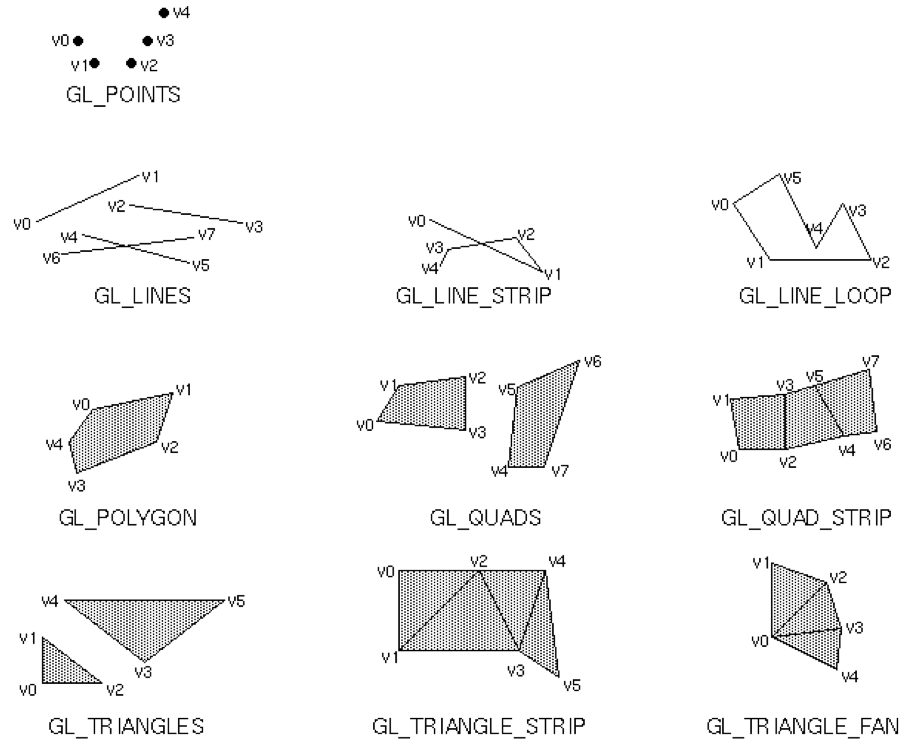
\includegraphics[width=0.5\textwidth]{glbegin} 
    \end{center} 
    \tiny
    Diagram: Copyright OpenGL Programming Guide. Addison-Wesley. 
    \normalsize
\end{frame} 

\begin{frame}{Mixing Geometry with Colour} 
    Specifying vertices can be mixed with colour and other 
    types of commands for interesting drawing results.
    \begin{columns}[t]
        \column{0.4\textwidth} 
        \showcode{geomcolor.c} 
        \column{0.6\textwidth} 
        \begin{center}
            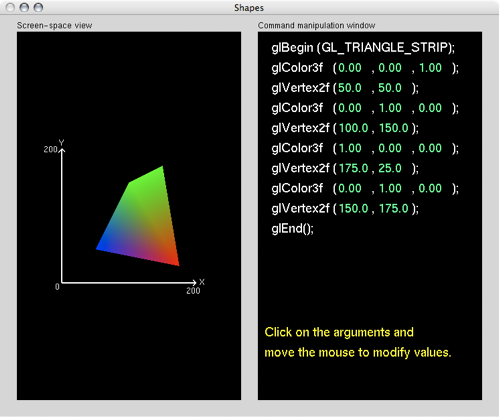
\includegraphics[width=0.6\textwidth]{geom-color} 
        \end{center} 
    \end{columns} 
\end{frame} 

\begin{frame}{Viewing the Scene: The Camera}
    \begin{center}
        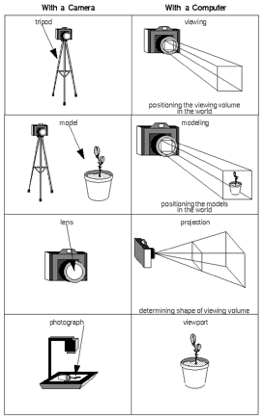
\includegraphics[width=0.3\textwidth]{camera} 
    \end{center} 
    \tiny
    Diagram: Copyright OpenGL Programming Guide. Addison-Wesley. 
    \normalsize
\end{frame} 

\begin{frame}{OpenGL Vertices} 
    \begin{itemize}
        \item OpenGL uses a 4-component vector to represent a vertex.
        \item Known as homogenous coordinate system~\footnote{For 
            further information on homogenous coordinate systems as 
            used in projective geometry and in OpenGL, see Appendix G of the Red Book
            \url{http://www.rush3d.com/reference/opengl-redbook-1.1/appendixg.html} } 
            where typically $w=1$.
        \item In 2D-space $z=0$.
    \end{itemize} 
    \begin{equation*}
        v = \left( 
                \begin{array}{c}
                x \\
                y \\
                z \\
                w
                \end{array}
            \right)
    \end{equation*} 
\end{frame} 

\begin{frame}{Vertex Transformations} 
    \begin{center}
        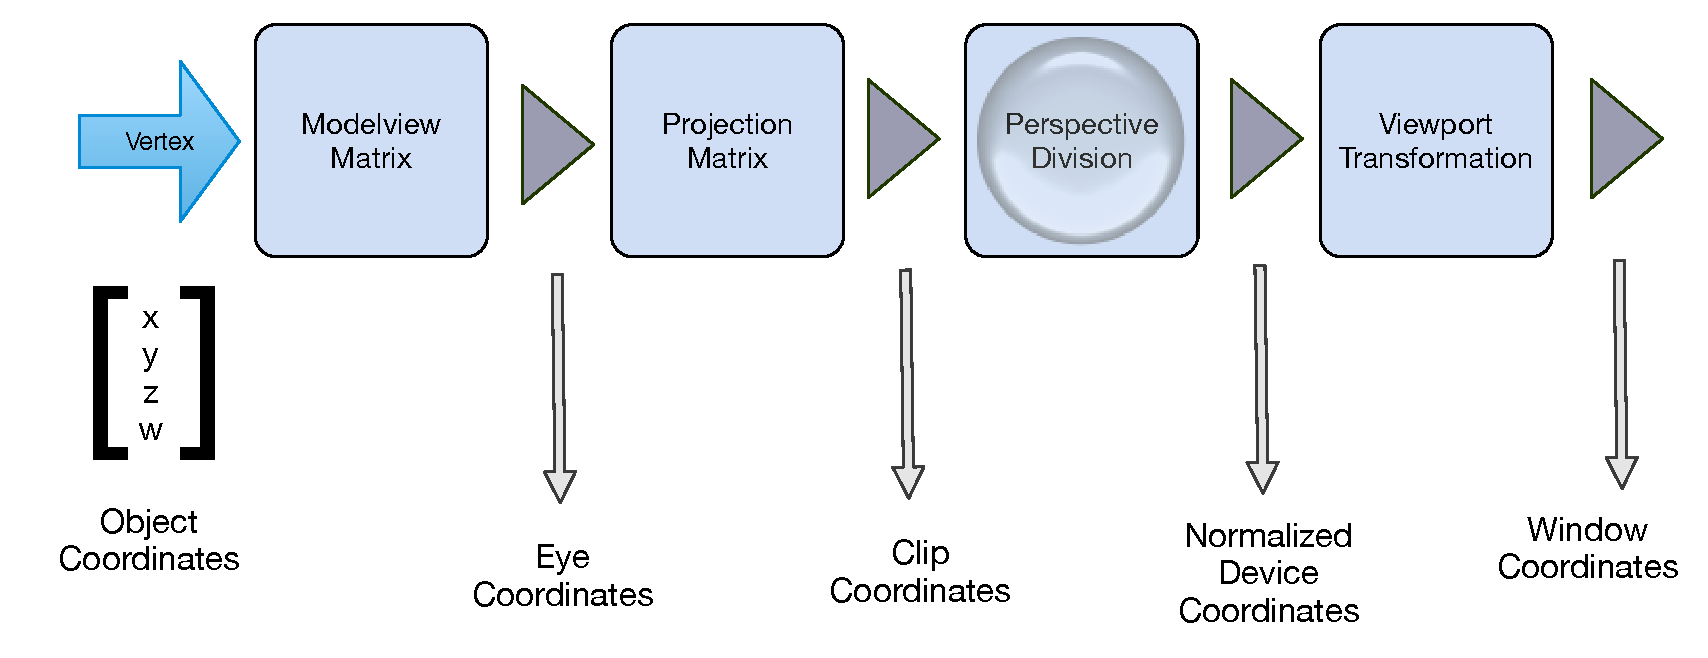
\includegraphics[width=\textwidth]{vertextransform} 
    \end{center} 
    \tiny
    Diagram adapted from the OpenGL Programming Guide. Addison-Wesley. 
    \normalsize
\end{frame} 

\begin{frame}{Vertex Transformation as Matrix Multiplication} 
    \begin{equation*}
        v' = M v
    \end{equation*} 
    \vspace{1cm} 
    \begin{equation*} 
        M = \left(
                \begin{array}{cccc}
                    m_{1}   & m_{5}     & m_{9}     & m_{13} \\
                    m_{2}   & m_{6}     & m_{10}    & m_{14} \\
                    m_{3}   & m_{7}     & m_{11}    & m_{15} \\
                    m_{4}   & m_{8}     & m_{12}    & m_{16} 
                \end{array} 
            \right)
    \end{equation*} 
\end{frame} 

\begin{frame}{The ModelView Matrix}
    \texttt{glMatrixMode(GL\_MODELVIEW);} \\[1cm]
    Specifying the \texttt{ModelView} matrix is analogous to:
    \begin{itemize} 
        \item Positioning and aiming the camera (viewing transformation)
        \item Positioning and orienting the model (modeling transformation)
    \end{itemize} 
\end{frame} 

\begin{frame}{The Projection Matrix}
\texttt{glMatrixMode(GL\_PROJECTION);} \\[1cm]
    \begin{itemize} 
        \item Specifiying the \texttt{Projection} matrix is like chosing a lens for a camera.
        \item It lets you specify parameters such as the field of view.
    \end{itemize} 
\end{frame} 

\begin{frame}{OpenGL Matrix Operations} 
    Identity Matrix
    \begin{equation*}
    I = \left(
                \begin{array}{cccc}
                    1   & 0     & 0     & 0     \\
                    0   & 1     & 0     & 0     \\
                    0   & 0     & 1     & 0     \\
                    0   & 0     & 0     & 1
                \end{array} 
            \right)
    \end{equation*} 
    \showcode{matrixops.c} 
\end{frame} 

\begin{frame}{Perspective Projection (glFrustrum)}
    \showcode{frustrum.c} 
    \begin{center}
        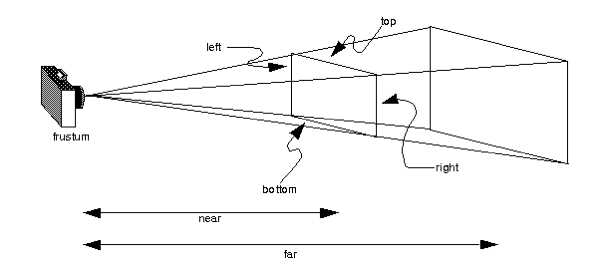
\includegraphics[width=0.8\textwidth]{frustrum} 
    \end{center} 
    \tiny
    Diagram: Copyright OpenGL Programming Guide. Addison-Wesley. 
    \normalsize
\end{frame} 

\begin{frame}{Perspective Projection (gluPerspective) from GLU} 
    \showcode{perspective.c} 
    \begin{itemize} 
        \item \texttt{fovy} : field of view in degrees, in the y direction
        \item \texttt{aspect} : aspect ratio that determines the field of view in
          the x direction (ratio of width to height)
    \end{itemize} 
    \begin{center}
        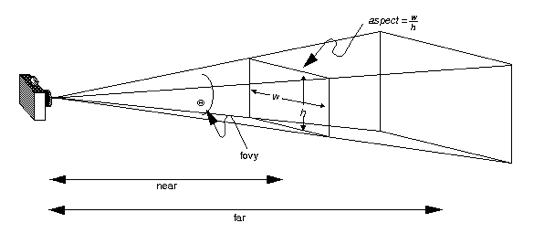
\includegraphics[width=0.5\textwidth]{perspective} 
    \end{center} 
    \tiny
    Diagram: Copyright OpenGL Programming Guide. Addison-Wesley. 
    \normalsize
\end{frame} 

\begin{frame}{Orthographics (Parallel) Projection - glOrtho} 
    \showcode{ortho.c} 
     \begin{center}
         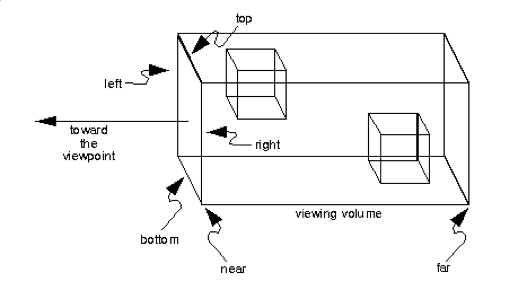
\includegraphics[width=0.6\textwidth]{ortho} 
    \end{center} 
    \tiny
    Diagram: Copyright OpenGL Programming Guide. Addison-Wesley. 
    \normalsize
\end{frame} 

\begin{frame}{gluLookAt}
    Specifies the camera position, the point where the camera is pointing, 
    and the orientation vector of the camera.
    \showcode{lookat.c} 
    \begin{center}
        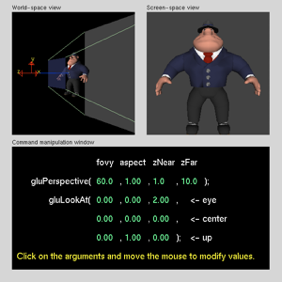
\includegraphics[width=0.3\textwidth]{lookat} 
    \end{center} 
    \tiny
    Screenshot from Nate Robin's OpenGL Tutors
    \url{https://user.xmission.com/~nate/tutors.html}
    \normalsize
\end{frame} 

\begin{frame}{Translation Transformation}
    \showcode{translate.c} 
    \begin{columns}[t]
        \column{0.5\textwidth}
            \begin{equation*}
                T = \left(
                        \begin{array}{cccc}
                            1   & 0     & 0     & x \\
                            0   & 1     & 0     & y \\
                            0   & 0     & 1     & z \\
                            0   & 0     & 0     & 1
                        \end{array} 
                    \right)
            \end{equation*} 
        \column{0.5\textwidth}
            \begin{equation*}
               T^{-1} = \left(
                        \begin{array}{cccc}
                            1   & 0     & 0     & -x \\
                            0   & 1     & 0     & -y \\
                            0   & 0     & 1     & -z \\
                            0   & 0     & 0     &  1
                        \end{array} 
                    \right)
            \end{equation*} 
    \end{columns} 
    \begin{equation*}
        v' = T v
    \end{equation*} 
    \begin{center} 
        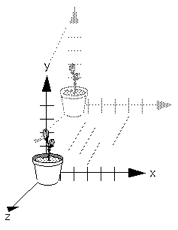
\includegraphics[width=0.15\textwidth]{translate} 
    \end{center} 
    \tiny
    Diagram: Copyright OpenGL Programming Guide. Addison-Wesley. 
    \normalsize
\end{frame} 

\begin{frame}{Rotation Transformations} 
    \showcode{rotate.c} 
    Specifies an angle and an axis (x,y,z) to rotate around.
    \begin{center} 
        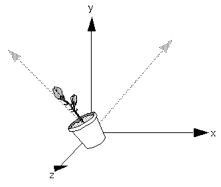
\includegraphics[width=0.3\textwidth]{rotation} 
    \end{center} 
    \tiny
    Diagram: Copyright OpenGL Programming Guide. Addison-Wesley. 
    \normalsize
\end{frame} 

\begin{frame}{Rotation Matrices} 
        \begin{equation*} 
        \texttt{glRotate3f($\alpha$, 1, 0, 0)} :
            R_x(\alpha) = \left(
                        \begin{array}{cccc}
                            1   & 0             & 0                 & 0 \\
                            0   & \cos(\alpha)  & -\sin(\alpha)     & 0 \\
                            0   & \sin(\alpha)  &  \cos(\alpha)    & 0 \\
                            0   & 0             & 0                 & 1
                        \end{array} 
                    \right)
        \end{equation*} 

        \begin{equation*} 
        \texttt{glRotate3f($\alpha$, 0, 1, 0)} :
            R_y(\alpha) = \left(
                        \begin{array}{cccc}
                            \cos(\alpha)    & 0             & \sin(\alpha)      & 0 \\
                            0               & 1             & 0                 & 0 \\
                            -\sin(\alpha)   & 0             & \cos(\alpha)      & 0 \\
                            0               & 0             & 0                 & 1
                        \end{array} 
                    \right)
        \end{equation*} 

        \begin{equation*} 
        \texttt{glRotate3f($\alpha$, 0, 0, 1)} :
            R_z(\alpha) = \left(
                        \begin{array}{cccc}
                            \cos(\alpha)    & -\sin(\alpha) & 0 & 0 \\
                            \sin(\alpha)    & \cos(\alpha)  & 0 & 0 \\
                            0               & 0             & 1 & 0 \\
                            0               & 0             & 0 & 1
                        \end{array} 
                    \right)
        \end{equation*} 
\end{frame} 

\begin{frame}{Scaling Transformations} 
    \showcode{scale.c} 
    \begin{columns}[t]
        \column{0.5\textwidth}
            \begin{equation*}
                S = \left(
                        \begin{array}{cccc}
                            x   & 0     & 0     & 0 \\
                            0   & y     & 0     & 0 \\
                            0   & 0     & z     & 0 \\
                            0   & 0     & 0     & 1
                        \end{array} 
                    \right)
            \end{equation*} 
        \column{0.5\textwidth}
            \begin{equation*}
               S^{-1} = \left(
                        \begin{array}{cccc}
                            \frac{1}{x} & 0             & 0             & 0 \\
                            0           & \frac{1}{y}   & 0             & 0 \\
                            0           & 0             & 1             & 0 \\
                            0           & 0             & \frac{1}{z}   & 1
                        \end{array} 
                    \right)
            \end{equation*} 
    \end{columns} 
    \begin{equation*}
        v' = S v
    \end{equation*} 
    \begin{center} 
        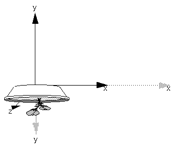
\includegraphics[width=0.2\textwidth]{scaling} 
    \end{center} 
    \tiny
    Diagram: Copyright OpenGL Programming Guide. Addison-Wesley. 
    \normalsize
\end{frame} 

\begin{frame}{Order of Transformations}
   \begin{center} 
       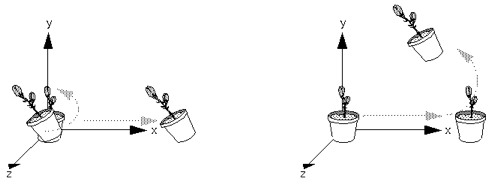
\includegraphics[width=0.7\textwidth]{order} 
    \end{center} 
    \tiny
    Diagram: Copyright OpenGL Programming Guide. Addison-Wesley. 
    \normalsize
\end{frame} 

\begin{frame}{Transformations in Action}
   \begin{center} 
       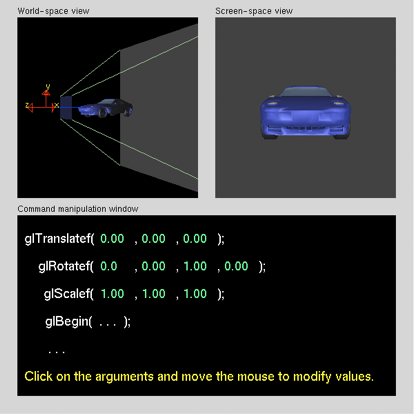
\includegraphics[width=0.4\textwidth]{action} 
    \end{center} 
    \tiny
    Diagram: Copyright OpenGL Programming Guide. Addison-Wesley. 
    \normalsize
\end{frame} 

\begin{frame}{The Matrix Stack} 
    \texttt{glPushMatrix()} and \texttt{glPopMatrix()} 
    \begin{columns}[t]
        \column{0.5\textwidth} 
        \showcode{matrixstack.c} 
        \column{0.5\textwidth} 
        \begin{center}
            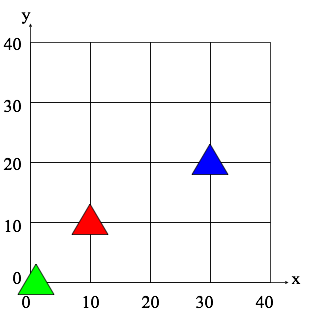
\includegraphics[width=0.5\textwidth]{stack} 
        \end{center} 
    \end{columns} 
\end{frame} 

\begin{frame}{OpenGL Lighting} 
    \begin{itemize} 
        \item Eight available lights (individually toggled)
        \item Lighting types:
        \begin{itemize} 
            \item Emitted
            \item Ambient
            \item Diffues
            \item Specular
        \end{itemize} 
        \item Material colours and properties
        \item Lighting demo
    \end{itemize} 
\end{frame} 

\begin{frame}{Setting up an OpenGL Light}
    \showcode{light.c} 
\end{frame} 

\begin{frame}{glLight\{if\}[v](light, pname, param)}
    \begin{center}
        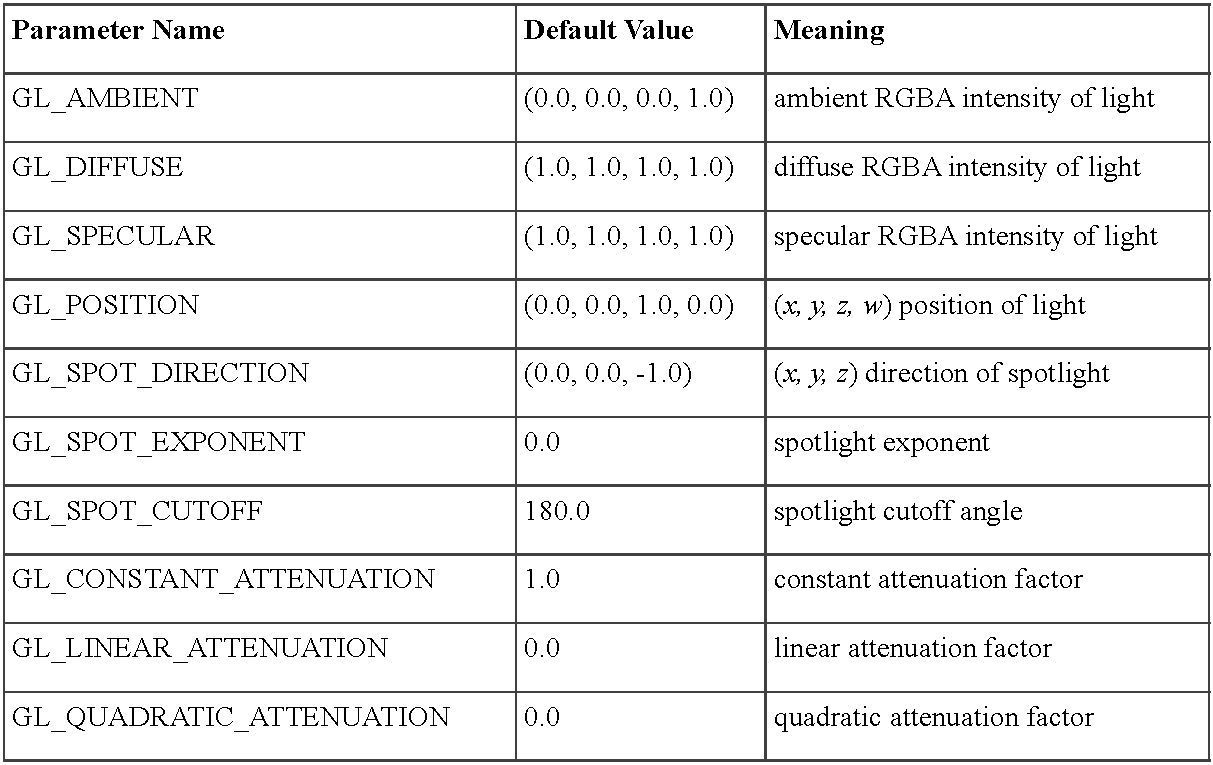
\includegraphics[width=0.8\textwidth]{gllight} 
    \end{center} 
\end{frame} 

\begin{frame}{Material Properties} 
    \texttt{glMaterial\{if\}[v](GLenum face, GLenum pname, TYPE param);} 
    \showcode{material.c} 
\end{frame} 

\begin{frame}{glMaterial Default Parameters} 
    \begin{center}
        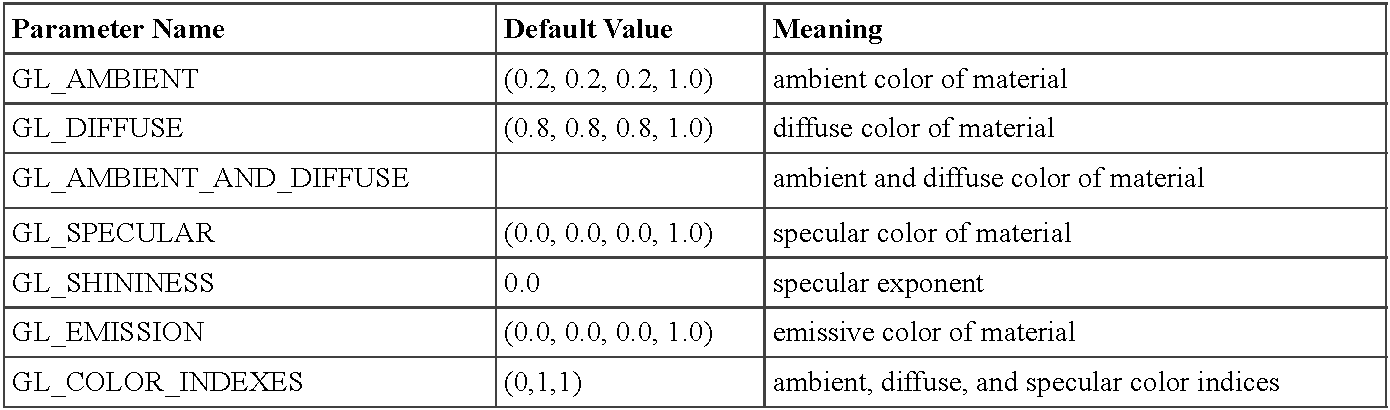
\includegraphics[width=0.8\textwidth]{materials}
    \end{center}
\end{frame} 

\begin{frame}{Teapots Materials Example} 
    \begin{center}
        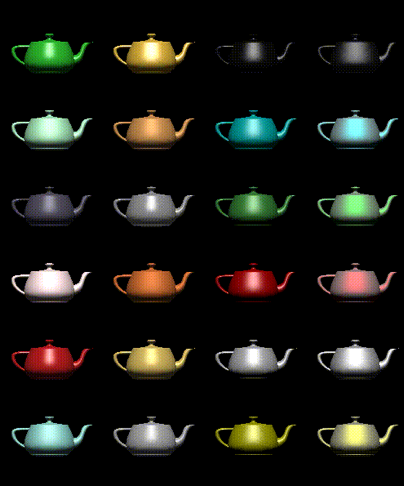
\includegraphics[width=0.4\textwidth]{teapots} 
    \end{center} 
    \tiny
    Diagram: Copyright OpenGL Programming Guide. Addison-Wesley. 
    \normalsize
\end{frame} 

\begin{frame}{Normal Vectors}
    \begin{center}
        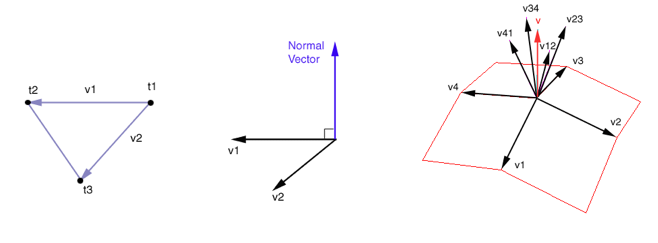
\includegraphics[width=\textwidth]{normalvectors} 
    \end{center}
\end{frame}

\begin{frame}{Normal Vectors -- \texttt{glNormal()}} 
    \showcode{normals.c} 
    \begin{center}
        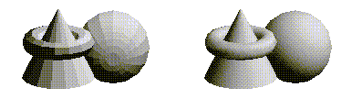
\includegraphics[width=0.5\textwidth]{smooth-vs-flat} 
    \end{center} 
\end{frame} 


\begin{frame}{Shading} 
    \begin{center}
        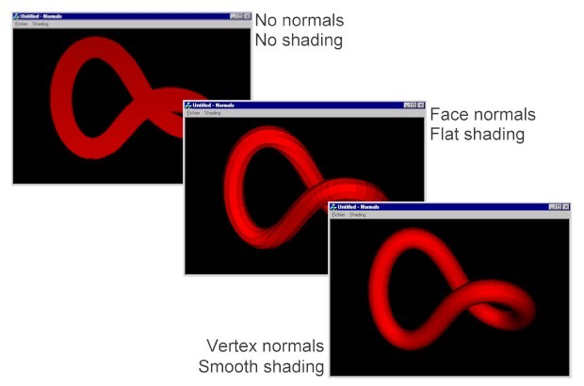
\includegraphics[width=0.6\textwidth]{shading} 
    \end{center}
    \tiny
    Diagram from:
    \url{http://www.codeguru.com/Cpp/G-M/opengl/article.php/c2681/} 
    \normalsize
\end{frame} 

\begin{frame}{Hidden Surface Removal} 
    In order for OpenGL to remove hidden surfaces, 
    you need to enable depth testing for the depth buffer.
    \showcode{hidden.c} 
\end{frame} 

\begin{frame}{GLUT} 
    \begin{itemize} 
        \item GLUT = GL UtilityLibrary
        \item Easy, stable, simple to use library for showing OpenGL demos.
        \item Limited to simple windows, mouse/keyboard input, and some simple 3D shapes.
        \item Most OpenGL demos and code on th eweb use GLUT.
        \item Default implementation in C
             (bindings for many languages available: Python, Perl etc)
    \end{itemize} 
\end{frame} 

\begin{frame}{Example GLUT Program in C} 
    \showsmallcode{glutmain.c} 
\end{frame} 

\begin{frame}{Typical InitGL() Function} 
    \showsmallcode{initgl.c} 
\end{frame} 

\begin{frame}{Typical GLUT Reshape Function} 
    \showcode{reshape.c} 
\end{frame} 

\begin{frame}{Typical GLUT Display Function} 
    \showcode{display.c} 
\end{frame} 

\begin{frame}{GLUT on Unix (command line)}
    \begin{block}{Compiling a GLUT Program on Unix/Linux}
    \small
    \texttt{gcc main.c -I/usr/X11R6/include -L/usr/X11R6/lib \\ -lGL -lGLU -lglut -lm}
   \normalsize
   \end{block} 

    On Unix or Linux systems includes should be:
    \showcode{unixincludes.c} 
\end{frame} 

\begin{frame}{GLUT on Mac OS X (command line) } 
    \begin{block}{Compiling a GLUT Program on Mac OS X} 
    \small
    \texttt{gcc main.c -F/System/Library/Frameworks  \\ -framework GLUT -framework OpenGL}
    \normalsize
    \end{block} 

    Using frameworks on Mac OS X, includes should be:
    \showcode{macincludes.c} 
\end{frame} 


\begin{frame}{OpenGL Books} 
    \begin{center}
        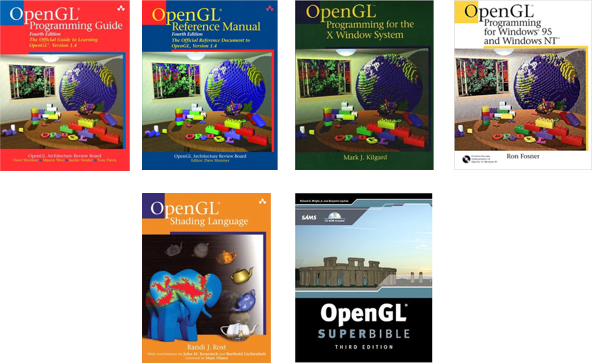
\includegraphics[width=0.8\textwidth]{books} 
    \end{center}
\end{frame} 

\begin{frame}{Resources} 
    \begin{itemize} 
        \item OpenGL Home Page \url{http://www.opengl.org}
        \item OpenGL Tutors \url{http://www.xmission.com/~nate/tutors.html}
        \item NeHe Tutorials: \url{http://nehe.gamedev.net}
        \item OpenGL Red Book (Programming Manual) \url{http://www.glprogramming.com/red/}
        \item OpenGL Blue Book (Reference Manual)
\url{http://www.glprogramming.com/blue/}
        \item Using GLUT with Visual C++ Express Edition

              \url{http://www.cs.rit.edu/~wrc/courses/common/cg1/doc/visual/GLUT_with_VCppEE.pdf}
    \end{itemize}
\end{frame} 

\end{document}
